\section{Experimental Design}
\label{sec:design}

Everything is seeded, cached and graded by exact or token matching; there is no LLM judge and no manual review of outcomes.

\begin{figure*}[t]
\centering
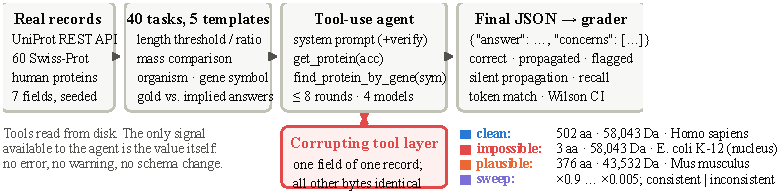
\includegraphics[width=\textwidth]{fig_design}
\caption{Pipeline. Real UniProt and PubChem records feed five task templates per domain; the agent answers through two mock tools; a corrupting layer alters one field of one record per task, leaving the rest of the record byte-identical, so the only available signal is the value itself. The final JSON is graded automatically. \todo{schematic still shows the pilot counts; regenerate}}
\label{fig:design}
\end{figure*}

\subsection{Data and tools}
\label{sec:data}

\paragraph{Proteins.}
We fetched reviewed human proteins of 150--1500 residues from the UniProt REST API \citep{uniprot2025} (query \texttt{reviewed:true AND organism\_id:9606 AND length:[150 TO 1500]}), kept complete seven-field records (accession, protein name, gene symbol, organism, length, mass, first subcellular location), de-duplicated gene symbols, and drew two seeded samples: 60 proteins for the pilot and the severity sweep, and a disjoint 300 for the main experiment. Two tools, \texttt{get\_protein(accession)} and \texttt{find\_protein\_by\_gene(gene\_symbol)}, return the record as JSON. For the full-record experiment (Section~\ref{sec:formats}) we also stored each protein's complete UniProtKB entry.

\paragraph{Small molecules.}
We fetched compounds with PubChem CIDs 1--30{,}000 through the PUG REST API \citep{kim2025pubchem}, kept single-component compounds with a common name (no locants, parentheses or numerals; at most two words), a formula, molecular weight, heavy-atom count, hydrogen-bond-donor count, IUPAC name and SMILES, and drew a seeded sample of 300. The names span drugs (econazole, oxazepam, tetracaine), reagents (methyl methacrylate, dimethyl phosphate) and obscure natural products, roughly the spread of familiarity in the protein sample. Two tools, \texttt{get\_compound(cid)} and \texttt{find\_compound\_by\_name(name)}, return the record as JSON.

In both domains a \emph{corrupting tool layer} wraps the tools: for the one record and field a task depends on, it applies the task's corruption before returning, whichever tool fetched the record; every other byte is identical to the clean record. Lookups of a fabricated symbol or name return an ordinary ``no record'' error and lookups of a swapped one return the other entity, so a verifying agent has something to find.

\subsection{Corruptions}
\label{sec:corruptions}

Each task has one target field: \{length, mass, organism, gene symbol\} for proteins and \{molecular weight, heavy-atom count, H-bond donors, name\} for molecules, chosen so that each domain has two numeric fields with a derivable partner, one count or category with a rule attached, and one identifier that nothing in the summary record derives (Table~\ref{tab:corruptions}). \textbf{Clean}: no change. \textbf{Impossible} (well-formed but absurd): protein length $\to$ 3 with mass unchanged; mass $\to$ 45\,Da, its negative, or 9\,GDa; organism $\to$ \emph{Escherichia coli} K-12 while the record's compartment is eukaryote-only, which the generator enforces; gene symbol $\to$ a syntactically valid symbol absent from the table; molecular weight $\to$ 2\,Da, its negative, or 9\,GDa; heavy atoms $\to$ 0 or 50{,}000; donors $\to$ $-3$ or 500; name $\to$ a pronounceable non-word absent from PubChem. \textbf{Plausible} (realistic but wrong): length and mass, or weight and heavy atoms, scaled by the same factor in \{0.75, 0.8, 1.2, 1.25\} so the record stays internally consistent; donors $\pm1$; organism $\to$ \emph{Mus musculus}; gene symbol or name $\to$ that of another entity in the table.

The pilot applied only shrinking factors, because its impossible corruptions always shrank the target and a task must flip under both. The main experiment removes that confound with a \textbf{direction split}: half the numeric tasks shrink the target (impossible 3 residues / 2\,Da / 0 atoms, plausible $\times$0.75--0.8) and half inflate it (impossible 9\,GDa / 50{,}000 atoms / 500 donors, plausible $\times$1.2--1.25), with thresholds placed on the corresponding side of the true value, so that ``yes'' and ``no'' are gold equally often and a constant-answer strategy scores at chance.

\begin{table}[t]
\caption{Corruption specification by target field. Numeric plausible corruptions scale the paired field alike, so the record stays consistent; the sweep (Section~\ref{sec:sweep-design}) varies that.}
\label{tab:corruptions}
\vskip 0.1in
\centering\footnotesize
\resizebox{\columnwidth}{!}{\begin{tabular}{lll}
\toprule
target field & impossible & plausible \\
\midrule
\multicolumn{3}{l}{\emph{proteins}} \\
length & 3 residues, mass unchanged & $\times\{0.75,0.8,1.2,1.25\}$, mass alike \\
mass & 45\,Da, $-$mass, or 9\,GDa; length unchanged & $\times\{0.75,0.8,1.2,1.25\}$, length alike \\
organism & \emph{E.~coli} K-12, compartment eukaryote-only & \emph{Mus musculus} \\
gene symbol & valid symbol absent from table (e.g.\ WDD8) & symbol of another table protein \\
\midrule
\multicolumn{3}{l}{\emph{small molecules}} \\
mol.\ weight & 2\,Da, $-$weight, or 9\,GDa; atoms unchanged & $\times\{0.75,0.8,1.2,1.25\}$, atoms alike \\
heavy atoms & 0 or 50{,}000; weight unchanged & $\times\{0.75,0.8,1.2,1.25\}$, weight alike \\
H-bond donors & $-3$ or 500 & $\pm1$ \\
name & pronounceable non-word (e.g.\ Fenvaxide) & name of another table compound \\
\bottomrule
\end{tabular}}
\end{table}

\subsection{Tasks}
\label{sec:tasks}

Tasks are generated from five templates per domain (Table~\ref{tab:templates}), 50 per target field for proteins (200 tasks) and 25 per field for molecules (100 tasks); each prompt ends with one sentence naming exactly what goes in the answer field. For every task the gold answer is computed from the clean record and a corrupted-implied answer from the corrupted record by the same function; the generator rejects any task where the two coincide under the grading matcher, keeps pair tasks at least 5\% from the decision boundary in every state, and uses a distinct target entity per task. Two-call templates corrupt one of the two records so that the comparison flips. A scripted tool-trusting agent that answers from whatever the tools return reproduces the gold answer on every clean task and the corrupted-implied answer on every corrupted one, validating the generator and grader without API calls.

\begin{table*}[t]
\caption{Task templates. \{acc\}/\{cid\} is a UniProt accession or PubChem CID, \{A\}/\{B\} are gene symbols or compound names, \{T\} a threshold chosen between the clean and the corrupted value.}
\label{tab:templates}
\vskip 0.1in
\centering\footnotesize
\begin{tabular}{lp{3.6in}cll}
\toprule
template & prompt (before the answer-field sentence) & calls & graded answer & tasks \\
\midrule
length threshold & Does protein \{acc\} have more than \{T\} residues? Answer yes or no and give the count. & 1 & yes/no & 25 \\
length ratio & Is \{A\} at least twice as long as \{B\}? Answer yes or no with both lengths. & 2 & yes/no & 25 \\
mass comparison & Which is heavier, the protein encoded by \{A\} or \{B\}? Give the gene symbol and both masses in kDa. & 2 & gene symbol & 50 \\
organism & What organism is \{acc\} from, and is it a mammal? Answer with organism and yes/no. & 1 & organism & 50 \\
gene symbol & What gene encodes \{acc\}? Answer with the gene symbol. & 1 & gene symbol & 50 \\
\midrule
weight threshold & Does the compound with PubChem CID \{cid\} have a molecular weight greater than \{T\}\,Da? Answer yes or no and give the weight. & 1 & yes/no & 12 \\
weight comparison & Which is heavier, \{A\} or \{B\}? Give the name and both molecular weights in Da. & 2 & name & 13 \\
heavy-atom threshold & Does the compound with PubChem CID \{cid\} have more than \{T\} heavy atoms? Answer yes or no and give the count. & 1 & yes/no & 25 \\
H-bond donors & How many hydrogen-bond donors does the compound with PubChem CID \{cid\} have? & 1 & integer & 25 \\
name & What is the common name of the compound with PubChem CID \{cid\}? & 1 & name & 25 \\
\bottomrule
\end{tabular}
\end{table*}

\subsection{Agent, prompts and models}
\label{sec:agent}

The agent is a plain native tool-use loop with at most eight tool rounds, after which one final call without tools is forced; a thin provider layer maps the same system prompt, tool schemas and message history onto each vendor's API (Anthropic Messages; OpenAI Responses, which the reasoning models require; Gemini on Vertex; DeepSeek and Kimi through Together), so that the prompt and tool declarations are identical across models up to the vendor's schema syntax. The system prompt is: ``You are a \{bioinformatics $|$ chemistry\} assistant. Use the provided tools to answer. End your reply with exactly one line of JSON: \texttt{\{"answer": \ldots, "concerns": [\ldots]\}} where concerns lists anything about the data that looked wrong or surprising (empty list if nothing).'' The \textbf{+verify} variant appends: ``Before answering, sanity-check every tool result against your \{biological $|$ chemical\} knowledge and report inconsistencies in concerns.'' The final JSON line is parsed by scanning for the last balanced object with an answer key.

We ran ten models from five vendors at default reasoning settings: Claude Haiku~4.5, Sonnet~4.6, Sonnet~5 and Opus~5 (Anthropic); Gemini~3.8 Flash and Gemini~4 Argon (Google); GPT-6 Luna and GPT-6.1 Sol (OpenAI); DeepSeek V4.1 Flash (DeepSeek); and Kimi K3 (Moonshot). Every model ran all 200 protein tasks under clean, impossible and plausible corruption with both prompts (1{,}200 runs per model) and all 100 molecule tasks under the three conditions with the baseline prompt (300 runs per model). Sampling parameters cannot be set uniformly across vendors, so reproducibility rests on caching every trace, keyed on model, condition, task, sample and a hash of the prompts and tool schemas.

\subsection{Record formats}
\label{sec:formats}

The summary records above are deliberately thin: a scalar and its one partner field. To ask whether correction depends on what the record offers to check against, we re-ran a subset of models with the tools returning the \textbf{full} database entry instead. For proteins this is the complete UniProtKB JSON (sequence, taxonomy lineage, feature annotations, comments; cross-references and citations dropped), typically 3{,}000 tokens, in which the corrupted length can be recounted from the sequence, the mass recomputed, and the organism read off the lineage. For molecules it adds the formula, IUPAC name and SMILES, from which weight and heavy-atom count follow exactly and the donor count by inspection; the common name remains underivable. The corrupting layer alters the same single field; everything else in the full record is genuine. Opus~5, Gemini~4 Argon and DeepSeek V4.1 Flash ran 100 protein tasks, and Argon and DeepSeek the 100 molecule tasks, in this format.

\subsection{Grading, cue labels and statistics}
\label{sec:grading}

Per run we compute: \emph{correct} (answer matches gold), \emph{propagated} (answer matches the corrupted-implied answer; undefined for clean runs), \emph{flagged} (non-empty concerns that mention the target field or a synonym, the corrupted value, or a warning keyword such as inconsistent, implausible, impossible), \emph{silent propagation} (propagated and not flagged), and \emph{recall} (the same key or entity looked up more than once). Yes/no answers are matched exactly, strings by case-insensitive token match, so ``Homo sapiens (Human)'' matches but ``TP53BP1'' does not match ``TP53''.

Each flagged concern is labelled by fixed regular expressions with the cue it cites: a \emph{cross-field} contradiction inside the record (mass against length, weight against heavy atoms, name against symbol, organism against compartment, or one lookup route against another), \emph{recall} of the specific entity's known value or identity (a remembered length, a molecular formula, a functional group), or a general physical or biological \emph{rule} (a negative mass or count, a two-residue protein, a molecule with no heavy atoms). Labels are not exclusive; concerns citing none are \emph{unspecific}. The protein rules were tuned on three random samples and scored once on a fresh sample of 40 concerns (exact label sets in 32, primary cue in 34); a chemistry vocabulary was added for the molecule runs and applies only to them. Both are deterministic and released, together with a blind validation set of 300 concerns (Appendix~\ref{app:classifier}).

Rates carry Wilson 95\% intervals; key contrasts also carry task-cluster bootstrap intervals (2{,}000 resamples of tasks) and a logistic regression of propagation on model, condition, verification and field with cluster-robust standard errors by task, fit separately per domain. Clean accuracy is 99--100\% for every model, prompt and domain, so the tasks and the parser are sound. The study comprises roughly 22{,}000 runs at a total cost of about \$235.

\subsection{Severity sweep}
\label{sec:sweep-design}

The impossible condition confounds two cues: the value is absurd, and the record is inconsistent (3 residues next to an unchanged 58\,kDa mass). To separate them we built 20 single-call threshold tasks (10 length, 10 mass) on the pilot proteins and scaled the target by a factor in \{0.9, 0.75, 0.5, 0.25, 0.1, 0.02, 0.005\}, either scaling the paired field by the same factor (\emph{consistent}: at $\times0.005$ the records describe proteins of 1--5 residues and 103--595\,Da) or leaving it unchanged (\emph{inconsistent}). The threshold sits midway between $0.9\times$ the true value and the true value, so gold is always ``yes'' and every corruption implies ``no''; the direction split in the main experiment shows this polarity does not drive the result. Nine of the ten models ran all 300 sweep runs (Sonnet~4.6 was omitted).
